% Converted from reference/DB4OTutorial (MadCap Flare, Java target)

\chapter{Object Manager}
\label{tut:object-manager}

The object manager allows us to open and explore db4o databases.

\section*{Installation}

The object manager is an Eclipse plugin. Its source code is in the enterprise/omj directory of the db4o repository; it is not built by the db4o build. Once you have built the plugin, start up Eclipse. There we choose 'Help'-\textgreater{}'Install New Software...'. Then we add the location of the unzipped object manager as an update site and continue the installation.

\begin{center}
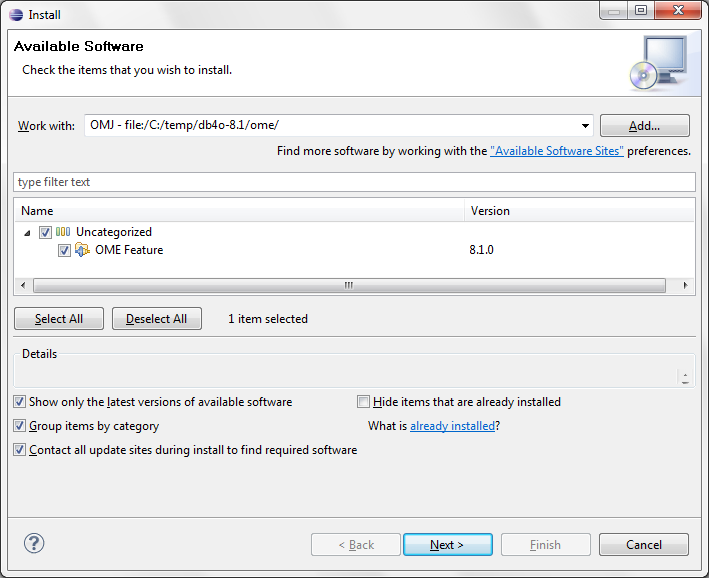
\includegraphics[width=\maxwidth]{images/tut-omj-installation.png}
\end{center}
\section*{Using the Object Manager}

To use the object manager we first open the OME perspective ('Window'-\textgreater{}'Open Perspective'-\textgreater{}'Other...'. Then we can open a db4o database.

After connecting we see a list of stored classes on the right. Below that we can inspect a stored class and see it details.

To query the database we drag and drop the fields we're interested in to the query builder. Then we change the condition and values on that query and run it.

\begin{center}
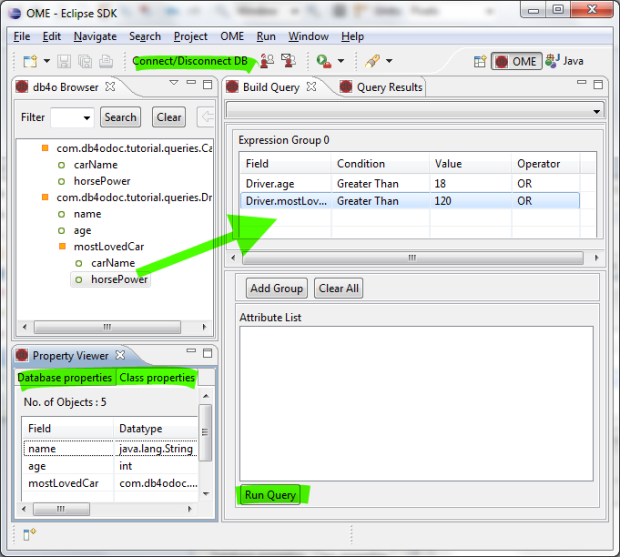
\includegraphics[width=\maxwidth]{images/tut-ome-overview.png}
\end{center}
On the result page we can select the different objects and inspect their values. We also can change values of objects and then store the data.

\begin{center}
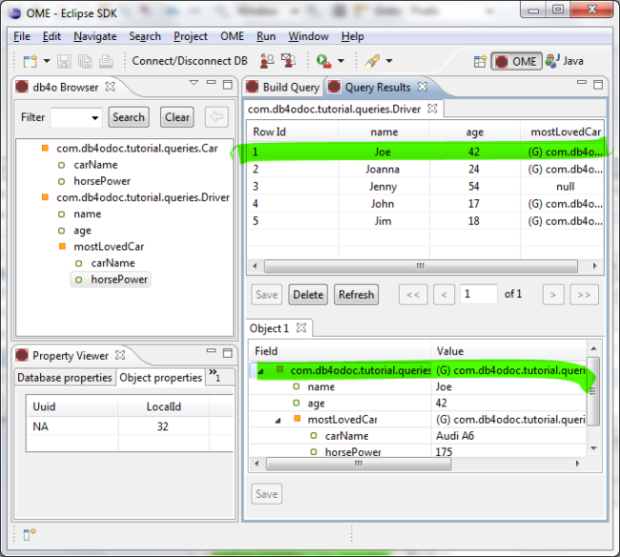
\includegraphics[width=\maxwidth]{images/tut-omj-result.png}
\end{center}
